\section{Results}\label{sec:short_results}

\subsection{When does posterior integration matter?}

Figure~\ref{fig:short_mechanism} shows when posterior integration changes option prices most in the simulated settings. The largest differences occur with short estimation windows, high volatility, long maturities, few realized fixings, and pronounced price curvature. Across the 10 million synthetic histories, the maximum observed absolute difference is 0.1565 for a normalized \$100 forward, and the highest 99th percentile among the simulated scenario groups is 0.1273. These extremes exceed the differences observed in the October-2026 sample. The maximum is sensitive to the number of simulations, while the 99th percentile is less affected by rare outcomes.

The second-order approximation tracks the simulated differences closely: the correlation between cell-level mean PI--PM differences and the curvature--variance term is 0.9995. Regressions constrained to pass through the origin also have slopes near one in the most extreme settings. These results support posterior variance and price curvature as the principal local determinants of the difference.

The PI--PM difference generally declines as the share of realized fixings increases. The change is not always steady: in Panel C, the 252-day case initially increases because known fixings affect both the remaining exposure to volatility and the curvature of the price function. The difference nevertheless tends toward zero as the averaging period ends.

\begin{figure*}[t]
\centering
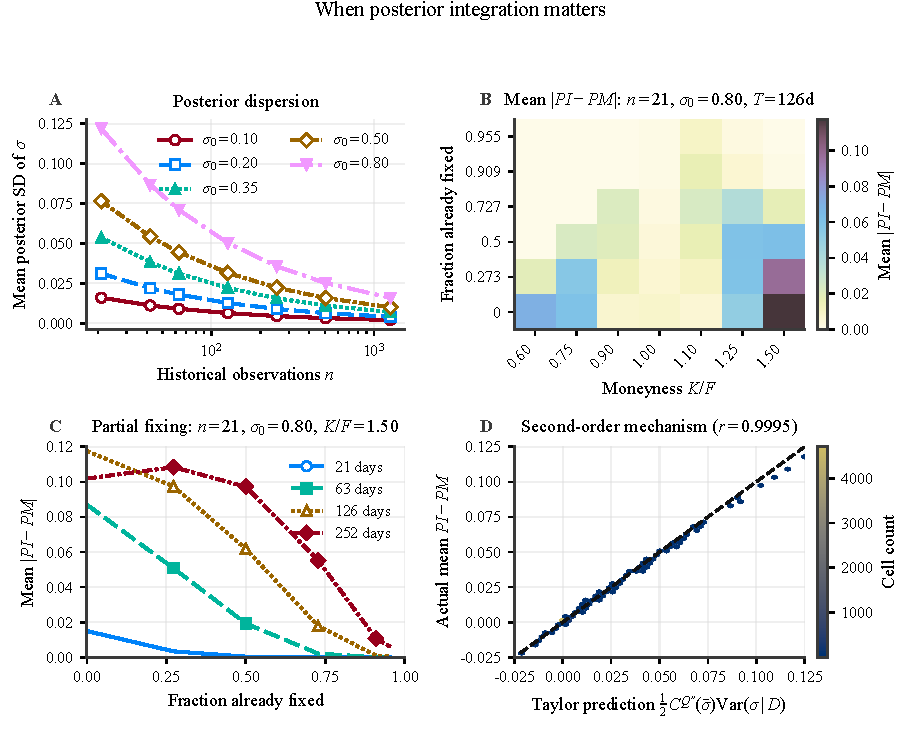
\includegraphics[width=\textwidth]{figures/publication/ten_million/fig01_mechanism_map.pdf}
\caption{Posterior integration across 10 million synthetic return histories and WTI-like option states (root seed 2468). Panel A shows posterior dispersion by historical sample size. Panels B and C show the absolute PI--PM difference across moneyness and the realized-fixing fraction. Panel D compares mean PI--PM differences for 5,880 scenario cells with the second-order approximation described in the methodology; the cell-level correlation is 0.9995. The color bar shows the number of scenario cells per hexagonal bin.}
\label{fig:short_mechanism}
\end{figure*}

\subsection{Posterior integration in the WTI sample}

The sample of options expiring in October 2026 contains 310 contract-date observations across 12 valuation dates from August 25 to September 10, 2026. Table~\ref{tab:short_october} shows nearly identical pricing errors for PI and PM (RMSE 0.5177 and 0.5183, respectively). Their mean absolute price difference is only 0.000745 dollars per barrel.

The central 95\% posterior interval for conditional model prices has mean width 0.2733 dollars per barrel, approximately 367 times the mean absolute PI--PM difference. The model prices vary across posterior volatility draws,
even though averaging those prices barely changes the point estimate.
This posterior interval does not describe forecast errors
against observed settlements or the value of an executable trade. Both methods underprice
the reported October settlement proxies on average.

\begin{table}[t]
\centering
\caption{WTI options with October 2026 expiry: posterior pricing and model-price uncertainty. Pricing error is model price minus settlement price. All price quantities and errors are in U.S. dollars per barrel.}\label{tab:short_october}
\begin{tabular}{lrr}
\toprule
Quantity & $N$ & Value \\
\midrule
PI RMSE & 310 & 0.5177 \\
PM plug-in RMSE & 310 & 0.5183 \\
Mean $|PI-PM|$ & 310 & 0.000745 \\
Mean 95\% posterior price-interval width & 310 & 0.2733 \\
\bottomrule
\end{tabular}
\end{table}

\subsection{Historical versus option-implied volatility}

Table~\ref{tab:short_forward} compares conditional pricing errors for 2,381 contract-date observations across just 15 valuation dates. The historical PI benchmark has MAE 2.6187 and RMSE 3.4090, compared with 0.1075 and 0.1594 for the previous-day APO implied-volatility smile. The expanding earlier-date smile performs similarly. Both specifications have lower errors than historical volatility in all seven expiries. Exploratory bootstrap intervals, calculated by resampling valuation dates, also lie below zero for each expiry (Figure~\ref{fig:short_forward_bootstrap}).

\begin{table*}[t]
\centering
\caption{Historical-volatility and earlier option-implied volatility comparisons. Panel A uses 2,381 contract-date observations over 15 valuation dates. Panel B uses only options with an earlier implied-volatility observation for the same contract. Historical PI uses Monte Carlo posterior integration; the other volatility inputs are priced using the same Curran approximation. MAE and RMSE are in U.S. dollars per barrel.}\label{tab:short_forward}

\textit{Panel A: date-ordered conditional pricing comparison}\\[2pt]
\begin{tabular}{lrrrr}
\toprule
Volatility input & $N$ & Dates & MAE & RMSE\\
\midrule
Historical PI & 2,381 & 15 & 2.6187 & 3.4090\\
Rolling 63 returns & 2,381 & 15 & 4.5201 & 5.6465\\
Horizon-matched GARCH(1,1) & 2,381 & 15 & 2.6730 & 3.4441\\
Previous-day APO implied-volatility smile & 2,381 & 15 & 0.1075 & 0.1594\\
\bottomrule
\end{tabular}

\vspace{5pt}
\textit{Panel B: same-contract lagged-IV benchmark}\\[2pt]
\begin{tabular}{lrrrr}
\toprule
Volatility input & $N$ & Dates & MAE & RMSE\\
\midrule
Historical PI & 2,366 & 15 & 2.6279 & 3.4173\\
Same-contract lagged IV & 2,366 & 15 & 0.0992 & 0.1403\\
Previous-day fitted APO smile & 2,366 & 15 & 0.1074 & 0.1594\\
\bottomrule
\end{tabular}
\end{table*}

Rolling-window, EWMA, and horizon-matched GARCH(1,1) estimates do not close the gap in pricing errors (Online Supplement Section S1 and Table S1).

Panel B isolates 2,366 observations with an earlier implied volatility for the same contract. Carrying that volatility forward yields lower pooled errors than the fitted previous-day smile (MAE 0.0992 versus 0.1074). On these matched observations, the improvement over historical
volatility does not require fitting an implied-volatility smile.
The 15 valuation dates are too few to establish that
carrying forward implied volatility generally outperforms
fitting a smile.

\begin{figure*}[t]
\centering
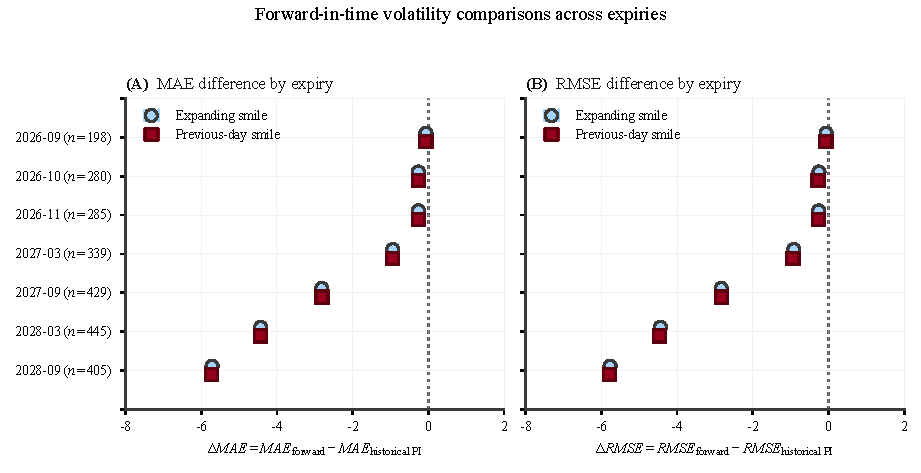
\includegraphics[width=\textwidth]{figures/publication/fig03_forward_q_cluster_bootstrap.pdf}
\caption{Date-ordered conditional pricing-error differences by APO expiry. Points compare the earlier-date APO implied-volatility specifications with the historical posterior-integrated benchmark; negative values indicate lower error for the implied-volatility specification. Horizontal bars are 95\% percentile intervals from valuation-date cluster bootstrap resampling. All implied-volatility inputs are dated before the valuation date in the archived records. We could not verify their original publication times or subsequent revisions.}
\label{fig:short_forward_bootstrap}
\end{figure*}

\subsection{Cross-instrument validation using vanilla-WTI options}

The cross-instrument comparison uses implied volatility from standard monthly WTI futures options instead of APOs. Table~\ref{tab:short_lo} uses 253 October-expiry APO contract-date observations across 10 valuation dates. Historical-volatility posterior integration has MAE 0.4464 and RMSE 0.5562. A previous-day vanilla-WTI implied-volatility specification based on LO options lowers these errors to 0.1559 and 0.2599. The corresponding previous-day APO implied-volatility smile has MAE 0.1676 and RMSE 0.2686.

\begin{table}[t]
\centering
\caption{Cross-instrument comparison for 253 October-expiry APO contract-date observations whose moneyness falls within the range covered by earlier LO option data. Historical PI is the canonical Monte Carlo posterior-integrated price; the vanilla-WTI and APO implied-volatility inputs are repriced with the deterministic Curran approximation. All implied-volatility inputs use only earlier-date option information. MAE and RMSE are in U.S. dollars per barrel.}\label{tab:short_lo}
\begin{tabular}{lrr}
\toprule
Volatility input & MAE & RMSE\\
\midrule
Historical PI & 0.4464 & 0.5562\\
Previous-day vanilla-WTI IV & 0.1559 & 0.2599\\
Previous-day APO IV & 0.1676 & 0.2686\\
\bottomrule
\end{tabular}
\end{table}

Valuation-date cluster bootstrap results support the improvement over historical volatility. Differences between LO-implied and APO-implied specifications are small and do not establish consistent superiority by MAE and RMSE. The result shows that earlier implied volatility also produces smaller errors when estimated from a different WTI option product.


\subsection{Extended conditional settlement-mark evidence}

The separate Databento analysis compares volatility inputs across
more valuation dates, but uses a different pricing model from
the earlier Curran analysis. Table~\ref{tab:remef_databento}
reports errors for the same observations classified
as actual settlements by the data provider. The previous-date
AAO implied-volatility benchmark gives an MAE of \$0.2184 per
barrel, versus \$0.8040 for posterior integration of the
historical volatility estimate based on earlier changes in
the average inferred from put--call parity. Both estimates
are evaluated within the same reduced-form terminal-average
approximation. Posterior integration itself changes historical
proxy pricing little: the PM MAE is \$0.8068.

\begin{table}[t]
\centering
\caption{Separate Databento AAO pricing comparison across 97,341 observations classified as actual settlements on 189 valuation dates. Errors are in dollars per barrel. The pricing model uses put--call parity estimates from other same-date strikes; it differs from the earlier Curran model based on CL fixing paths.}
\label{tab:remef_databento}
\begin{tabular}{lrr}
\toprule
Volatility input and pricing method & MAE & RMSE\\
\midrule
Earlier AAO option-implied volatility & 0.2184 & 0.2979\\
Historical proxy, posterior integration & 0.8040 & 1.1372\\
Historical proxy, posterior-mean plug-in & 0.8068 & 1.1401\\
\bottomrule
\end{tabular}
\end{table}

The difference is consistent with the fact that historical
changes in the expected average and option-implied volatility
of the terminal average measure different quantities.
For comparison, we infer implied volatility retrospectively from
near-the-money options on the valuation date. Its mean is 30.97\%
across 1,689 expiry-date groups, compared with 26.68\% for the
volatility equivalent to the Bayesian plug-in price and 30.88\%
for earlier AAO implied volatility.
The target-date inversion is used \emph{only to diagnose} pricing
errors after scoring, never as an input to forecasts. These
numbers do not identify a volatility risk premium.

Table~\ref{tab:remef_bayes_iv} asks whether Bayesian modeling
of earlier implied volatility improves on simply carrying
forward the last observed value, using the same prior
option-market information. On 47,718 observations classified as actual settlements across
88 dates in 2025--September 2026, it does not. Carrying forward the last implied volatility gives slightly
lower MAE and RMSE. Posterior integration and pricing at the
Bayesian posterior mean give nearly identical errors. The estimated improvement in daily MAE from Bayesian updating,
averaging equally across valuation dates, is -\$0.00100/bbl.
A 95\% bootstrap interval obtained by resampling calendar months
is [-\$0.00331,\$0.00082].
The interval crosses zero. The observed differences are too small and uncertain to
support a claim of economic advantage.

\begin{table}[t]
\centering
\caption{Pricing comparison for 47,718 AAO observations classified as actual settlements across 88 valuation dates from 2025 to September 2026. Bayesian estimates use option-implied volatility recorded on earlier dates.}
\label{tab:remef_bayes_iv}
\begin{tabular}{lrr}
\toprule
Method & MAE & RMSE\\
\midrule
Unchanged earlier-date AAO implied volatility & 0.2089 & 0.3014\\
Bayesian market-IV posterior-mean plug-in & 0.2098 & 0.3023\\
Bayesian market-IV posterior integration & 0.2098 & 0.3024\\
\bottomrule
\end{tabular}
\end{table}

A separate analysis tests the coverage of intervals for
settlement-price errors using 89,696 observations classified as
actual settlements across 174 dates after an initial estimation period. In the inspected 2025--September 2026
subset, the Bayesian model for pricing errors, combined with the
Bayesian implied-volatility price, achieves 86.43\% coverage for
nominal 90\% intervals and 90.11\% coverage for nominal
95\% intervals. Intervals based on rolling empirical error quantiles,
with equal weight across dates, cover 84.72\% and 90.66\%,
respectively. Comparisons of interval scores using calendar-month
resampling show no consistent Bayesian advantage. The coverage changes substantially over time:
nominal 90\% Bayesian intervals cover only 59.0\% and
56.9\% of targets in March and April 2026, respectively.
These are intervals for \emph{errors against settlement prices},
not the posterior ranges of \emph{model prices} reported earlier.
The two intervals describe different kinds of uncertainty.
